\chapter{Antecedentes}

% este apartado podría tener un orden: de lo más lejano a lo más cercano

% Aquí pienso colocar los antecedentes del proyecto.
% Me pregunto sobre la pertinencia de escribir una especie de estado del arte.
% Había pensado hablar de algunos proyectos cercanos que influyen en el proyecto
% Esto aparece ligeramente enunciado en el artículo de Panorama y en el texto que preparé para el coloquio
% Podría hacer un seguimiento al trabajo que hacen personas cercanas
% Incluso aquí podrían ir los primeros ejercicios en la web 
% Me imagino que aquí podrían aparecer algunos registros anectóticos 

Los antecedentes de esta investigación aluden a una trayectoria que va de la transición de la escritura de software para la realización de sistemas interactivos a la escritura de módulos de software audiovisuales. Estas experiencias toman como premisas la optimización y la ligereza de hardware (por ejemplo, con el uso de computadoras de placa reducida como Raspberry Pi o Jetson Nano ) y la elaboración sistemas ligeros, accesibles y portables para la síntesis y renderización audiovisual en el navegador.

A la par de la práctica artística con tecnología, los elementos precedentes de esta investigación se han conducido hacia la problematización del software como una instancia tanto de conocimiento como de ideas que conforman un paradigma que atraviesa todo el entramado de personas, investigaciones, escritos y obras involucrado con esta actividad. Estas reflexiones han tenido eco en el campo de investigación denominado estudios del software.

Los antecedentes a continuación descritos no necesariamente tienen un orden cronológico o de importancia. En todo caso es un compendio de perspectivas, plataformas, obras y realizaciones prácticas que desde la perspectiva de quien suscribe este texto, son relevantes de enunciar para captar las incidencias en los casos de investigación. 

\section{Antecedentes de Investigación}

\textit{Tres Estudios Abiertos} es resultado de proyectos de investigación previos. 

% \subsection{Objeto, Paisaje y Efecto}

\emph{Objeto, Paisaje y Efecto}\citep{ocelotlLic} fue un proyecto de investigación que abordó las nociones de objeto sonoro \citep{schaeffer}, paisaje sonoro\citep{schafer1} y efecto sonoro \citep{augoyard} para considerar a la escucha como un recurso para la investigación sociológica en música y para la investigación social desde el sonido. Este último aspecto marco el salto de la investigación que parte de una observación distanciada a la intención de incorporar conceptos de otras disciplinas para la investigación en ciencias sociales pero también para la reflexión sobre el cruce entre música y tecnología. Rescato esta investgación en lo que respecta a la postura hacker en tanto que actitud para apertura y aprendizaje con dispositivos que no necesariamente se ciñen a lo tecnológico, sino que también pueden problematizar las relaciones sociales que existen en la triada performática que existe entre compositores, escrituras tecnológicas e instrumentistas.  

% \subsection{Cuidado con la Brecha}

Un segundo punto de investigación fue \emph{Cuidado con la brecha}. Esta investigación involucró un proceso de investigación-producción artística \citep{ocelotlMas}. La realización de este proyecto fue un prototipo tecnológico y partió de objetivos que inicialmente estaban propuestos como secundarios pero que más tarde se revelaron como parte del núcleo en la investigación. Estos aspectos son: 1) el proceso de trabajo colaborativo y su implementación con herramientas como git, 2) la reflexión sobre la interacción entre audio e imagen en la composición musical electroacústica y 3) el uso de herramientas libres, personalizadas para la realización de prototipos audiovisuales y para el planteamiento de una observación crítica de procesos creativos donde investigador y artista son el mismo agente. La propuesta de los estudios del software fue incorporada en este momento de investigación. 

% \subsection{Tres Estudios Abiertos}

Desde la óptica de la escritura de software, esta investigación conecta y retoma algunas ideas que han sido plasmadas anteriormente. Estas fueron incorporadas como elementos secundarios que acompañan el objetivo principal de esta investigación: La visibilización de las contradicciones en la escritura de software como pregunta de investigación y como motivo para la realización artística.

%\section{Trilogía de Investigación}

%\textit{Tres Estudios Abiertos} forma parte de una trilogía de investigación. 

%\subsection{Objeto, Paisaje y Efecto}

%La primera parte fue Objeto, Paisaje y Efecto \citep{ocelotlLic}, un proyecto de investigación que abordó las nociones de objeto sonoro \citep{schaeffer}, paisaje sonoro\citep{schafer1} y efecto sonoro \citep{augoyard} para considerar a la escucha como un recurso para la investigación sociológica en música y para la investigación social desde el sonido.

%\subsection{Cuidado con la Brecha}

%Un segundo punto de investigación involucró un proceso de investigación-producción artística \citep{ocelotlMas}. La realización de este proyecto fue un prototipo tecnológico y partió de objetivos que inicialmente estaban propuestos como secundarios pero que más tarde se revelaron como parte del núcleo en la investigación. Estos aspectos son: 1) el proceso de trabajo colaborativo y su implementación con herramientas como git, 2) la reflexión sobre la interacción entre audio e imagen en la composición musical electroacústica y 3) el uso de herramientas libres, personalizadas para la realización de prototipos audiovisuales y para el planteamiento de una observación crítica de procesos creativos donde investigador y artista son el mismo agente. La propuesta de los estudios del software fue incorporada en este momento de investigación. 

%\subsection{Tres Estudios Abiertos}

%Referencia recursiva a esta investigación para explicar la trilogía

% \section{Música por computadora y algorítmica} % Esto se podría contradecir con el capítulo de marcos, peinso que esto se podría ir de aqui igual que el apartado de live coding 

%\subsection{Documenta X} % Pendiente tal vez podría ir en las conclusiones o como una problemmatización een la parte de montaje de anti

%Conexiones y accesos en muestras que implican espacios físicos y digitales. 

%\subsection{Plataformas}


%A continuación, haremos un breve rastreo de ideas centrales en la escritura de software orientado a la creación musical. El objetivo de este apartado consiste en describir y detectar la presencia del concepto unidad generadora en diversos programas orientados a la generación musical, de entre los cuales está una de las librerías que la presente investigación implementa.

%El punto de partida de esta indagación es MUSIC N, proyecto de Max Mathews que sería el parteaguas del paradigma de la música por computadora. Uno de los primeros casos de esta instancia es el principio de programas como Max/MSP y PureData, proyectos representativos de la programación gráfica presente en flujos de trabajo gráfico actuales como TouchDesigner.

%Como una observación adicional, es importante detectar instancias de la programación gráfica y de las ideas principales de la música por computadora en plataformas con giros programáticos particulares. Tal es el caso de OpenMusic, que de manera específica está basado en Common Lisp.

%Desde la perspectiva de la programación escrita, destacamos el papel que ha tenido SuperCollider en la extensión del paradigma de la música por computadora en la actualidad. Señalamos la importancia de SuperCollider como el motor bajo el cual se pueden ejecutar entornos de programación al vuelo como Tidal Cycles o FoxDot. 

%Estuary es un caso adicional que permite establecer un puente entre Tidal Cycles como un entorno que ejecuta SuperCollider como motor de audio y el navegador como tecnología multiplataforma sin instalaciones. Esta plataforma utiliza secuenciadores basados en la sintaxis de Tidal Cycles pero a diferencia del entorno que se puede instalar de manera local en una computadora, Estuary utiliza al navegador como motor de audio. 

%Trazamos estas relaciones para establecer una relación continua y presente entre los entornos anteriormente descritos y una de las librerías utilizadas en los casos de estudio de esta investigación: Tone.js. En este sentido, consideramos importante la adscripción a los principios de la música por computadora para encontrar soluciones personalizadas para el navegador.

%\subsection{Jacktrip y la música conectada}

%Una parte de los antecdentes de este proyecto se vinculan con la actividad del colectivo RGGTRN\footnote{\url{https://rggtrn.github.io/}. Consultado el \today} y del LiveCodeNet Ensamble\footnote{\url{https://livecodenetensamble.wordpress.com/}. Consultado el \today}

%RGGTRN es un colectivo de música por computadora fundado por Luis N. Del Angel y Emilio Ocelotl. Posteriormente se unieron Marianne Teixido y Jessica A. Rodríguez. Como parte de un ejercicio lúdico y de reflexión, el colectivo explora la improvisación audiovisual realizada por medio de código de programación, con una relación al contexto Latinx de sus participantes.

% Tesis de Luis
% Bellacode
% Saborítmico
% Tesis de maestría de hernani
% Artículo de Hernani n algún lado
% Artículos de Jessica ? 

%raspis conectadas y jacktrip > el trabajo realizado por CCRMA y en general 

%La labor del colectivo Radiador

% La radio y la transmisión de sonido con Icecast 

%Sonobus y la resolución de problemas de streaming en tiempos de pandemia

%\subsection{Fluxus y openGL}

%Para el caso de la imagen, retomo la influencia que tiene en la comunidad de live coding y en mi experienciación del performance audiovisual con la computadora el papel que tuvo el desarrollo Fluxus\footnote{\url{https://gitlab.com/nebogeo/fluxus/}} de Dave Griffiths que se remonta al 2007. Una característica peculiar de este desarrollo es el uso de una sintaxis tipo LISP que recuerda a desarrollos musicales basados en este lenguaje de programación como OpenMusic. 

%Detrás de Fluxus también cabe destacar la importancia de sistemas de renderización de gráficos por computadora como OpenGL, que actualmente, son el punto de partida de software de alto nivel involucrado con este proyecto como OpenFrameworks y la variante para el navegador, webGL, que implementa la librería Three.js 

% Pregunta, esto no tendría que ir en otros momentos? Tal vez disperso o tal vez en la introducción 

%\section{Live Coding} % Pregunta: Este apartatdo no debería ir antes ? En momentos anteriores menciono la cuestión  

% Antecedentes más extensos

%Encuentro múltiples formas de abordar el tema. El live coding puede describirse en térrminos de unaa comunidad que realiza una práctica y que se enuncia como tal, como un sub-campo creativo que comparte elementos con otra expresiones como la música algorítmica y el arte generativo. Finalmente, el live coding podría acotarse a motivos de investigación académica e independiente y a la realización tecnlógica de interfaces de texto que corren sobre motores de audio y video.

%De estas múltiples formas de abordar el fenómeno y de acuerdo a los fines de esta investigación, nos preguntamos si el eje que las articula son discusiones sobre el lenguaje y la escritura. 

%\subsection{Primeras expresiones}

%Antecedentes del live coding: la escena mod.

%En el manifiesto del live coding se expresan pensamientos que hasta el momento, son vigentes. 

% PhD Thesis: Artist-Programmers and Programming Languages for the Arts - Alex McLean 
%Dentro de los antecedentes está la experiencia performática de escribir código al vuelo con fines creativos, audiovisuales y experimentales.

%Las primeras expresiones reflexivas y prácticas del live coding no solamente establecen puntos de partida performáticas, sino que al mismo tiempo aportan elementos para el diseño y análisis de sistemas basados en interfaces de código:

%\begin{quote}

%  ``Nuestro argumento nos lleva a través de capas de representación, comenzando con símbolos, luego palabras, lenguaje y notación, para considerar el papel que estas representaciones pueden jugar en la creatividad humana'' \citep[p.~3]{McLean2011}

%\end{quote}

%La noción de capas de representación permite analizar la complejidad del proceso artístico con código en términos de la relación entre humanos y los aspectos cognitivos, sociales y políticos que les atraviesan, y los no-humanos en lo que respecta a las posibilidades de conocimiento instanciado presentes en ellos. 

%Live coding desde cero y la improvisación. 

%\subsection{Nodos y circuitos}

%La práctica de la programación al vuelo, delimitada técnica, escénica, musical y visualmente se origina en Inglaterra. % cita

%Como lo describen \cite{villasenor} para los casos de Barcelona y Ciudad de México.\footnote{Un ejemplo reciente se encuentra en: \url{https://youtu.be/n5kwi4eRAE4}} 

%\subsection{Exploración visual}

%Exploración visual para la integración con el sonido.  

%\begin{figure}[tb]
%\centering 
%\includegraphics[width=\columnwidth]{../img/of13.png} 
%\caption[Openframeworks 1]{Captura de render realizado con OpenFrameworks} % The text in the square bracket is the caption for the list of figures while the text in the curly brackets is the figure caption
%\label{fig:gallery} 
%\end{figure}

%El campo del live coding tuvo un giro importante con la llegada de hydra de Olivia Jack. La rápida expansión de esta plataforma y la sintaxis que recuerda la conexión de flujos de energía similar a los sintetizadores analógicos favorecieron la producción de piezas e interpretaciones enfocadas en la imagen y en algunos otros casos a la par del audio. La importancia de esta plataforma ha delimitado una estética  basada en  la transformación de píxeles, de formas y de transformaciones basadas en funciones matemáticas.

%En palabras de Olivia Jack, los procesos que realiza la computadora hay un eje de profundidad, en términos del despliegue gráfico físico de la computadora de espacios bi o tridimensionales, el resultado es bidimensional.

%La lógica de Hydra es modular, esto quiere decir que puede incorporarse como un componente adicional a proyectos que no necesariamente se centren en la producción visual con esta plataforma. Esta modularidad juega a favor de lenguajes de programación como Javascript. 

\section{Niveles, ecosistemas y fuera de línea}

Los proyectos cercanos tecnológica, conceptual y estéticamente a esta investigación se pueden dividir en cinco rubros: por un lado, nivel bajo, medio y alto dependiendo de la cercanía con el lenguaje de la máquina y por el otro, ecosistemas y proyectos fuera de línea.

Las plataformas y marcos de trabajo utilizados en esta investigación son problematizados a profundidad en capítulos siguientes; el resto, puede ser considerado con un conjunto de proyectos colindantes. Los casos, al ser ordenados de bajo a alto nivel, también describen una trayectoria de realización de prototipos de las piezas que forman parte de esta investigación.

Un cuarto conjunto de proyectos describen esfuerzos por mantener la diversidad sintáctica en los lenguajes de programación de alto nivel, fungiendo como contenedores que permiten la renderización de audio y en algunos casos, de vido, a partir de esta sintaxis.

Consideramos un último rubro de proyectos tecnológicos que permiten este tipo de realización audiovisual: aquel que se desenvuelve fuera de línea y que ha sido un punto de partida para la práctica performática audiovisual que también sirve como antecedente para el presente trabajo. 

A continuación, un listado de proyectos que contempla con estas premisas y una descripción que las relaciona con esta investigación. 

\paragraph{Nivel bajo}

Destaca por la optimización pero también por la complejidad en la escritura de código. Algunos proyectos que colindan con esta investigación son: 

%\subsection{Nivel Bajo}

\begin{itemize}

\item \Gls{WASM} o WebAssambly es una alternativa a la compilación con lenguajes de programación dedidcados al navegador. Por ejemplo, es posible realizar una aplicación en OpenFrameworks y compilarla para que pueda funcionar en el navegador.  
\item \Gls{rust} es un lenguaje de programación que permite compilar a WebAssembly. La indagación realizada con el siguiente proyecto permitió tener en cuenta este lenguaje de programación en la medida que permite acceder a funciones de bajo nivel sin perder flexibilidad.  
\item \Gls{ruffbox} es un proyecto escrito por Niklas Reppel en el lenguaje de programación Rust. Considero que este proyecto es de suma utilidad para la presente investigación ya que es un caso de realización de bajo nivel para el navegador con una sintaxis y lógica personalizadas. 
\item Flocking\footnote{\url{https://github.com/continuing-creativity/Flocking/}}
\end{itemize}

%\subsection{Nivel Medio}

\paragraph{El nivel medio} supone herramientas que tienen funcionalidades determinadas y que no requieren que las instrucciones tengan que ser escritas con un nivel de abstracción inferior. Cabe destacar que una parte importante de la experiencia inicial con el trabajo con audio y video en la web descansa en este tipo de proyectos. Por lo general, tienen funciones y posibilidades que solucionan problemas comunes como cargar un objeto tridimensional previamente diseñado o reproducir un archivo de audio. Este nivel es abordado a profundidad en el siguiente capítulo, a continuación, una descripción breve y su posible relación con esta investigación y el resto de los antecedentes. 

\begin{itemize}
  
\item \Gls{webaudio} Es una especificación para realizar audio en el navegador. Hasta el momento, los módulos de código escritos dentro de esta investigación parte de este proyecto ya que permite enlazarlos con módulos de más alto nivel y tamabién permite realizar modifcaciones en estructuras de procesamiento de audio que son similares a los Generadores Unitarios.
\item \Gls{tonejs} fue una librería que este proyecto implementó para tener un mayor control en el procesamiento de audio. Si bien la librería es limitada, permite resolver problemas de audio con una curva de aprendizaje relativamente corta. Algunos problemas de secuenciación y de distribución de eventos en el tiempo se resuelven de manera eficiente. Por este motivo, las estructuras que permiten generar patrones son utilizadas como estructuras de control temporal en las piezas que se han mencionado anteriormente.
\item \Gls{threejs} es una plataforma para generar gráficos en 3d. Cuenta con algunos módulos para reproducir audio y posicionar la escucha en algun lugar de este espacio tridimensional. Esta aproximación fue la primera que el presente proyecto realizó, ya que la integración con la librería de imagen prácticamente estaba resuelta. Estas características son suficientes para reproducir pero son limitadas para procesar audio. 
\item \Gls{supercolliderjs} y \Gls{supercolliderweb} son casos que se integran con SuperCollider desde el navegador. Con este plataforma no es posible compilar y ejecutar un servidor de SuperCollider en el navegador o en algún servidor conectado a la web, sin embargo, sirve como punto de partida para hablar de los proyectos que compilan SC desde el navegador y que aprovechan las posibilidades de las aplicaciones web.

\item maximilian 
  
\end{itemize}

%\subsection{Nivel Alto y Ecosistemas}

%\subsubsection{Nivel Alto}

\paragraph{El nivel alto} implica que las funciones convencionales para el tratamiento de audio y video están resumidas en una sintaxis que permite llegar a resultados complejos y delimitados con pocas líneas de código. Por lo general, este nivel permite la interpretación al vuelo del código y posibilita el uso del código en presentaciones en vivo. Bajo ciertas circunstancias, podría comparar este nivel alto con el resultado del trabajo de un artesano. Considero que este nivel es el más interesante de analizar ya que permite observar las intenciones estéticas y políticas en decisiones sintácticas de alto nivel. Algunas de ellas pueden perseguir expresiones convencionales que van de la renderización de ruido sin pasar por la construcción desde cero de una función matemática a la reproducción de patrones rítmicos con muestras de audio que coinciden  con los estilos de la música latinoamericana para la pista de baile. % Por acá podría poner lo de Dijskra y el otro sujeto que escribe alphabet creo 

Algunos proyectos que cumplen con estas características son: 


\begin{itemize}
\item \Gls{hydra} es una inspiración directa para este proyecto. Cumple con la premisa del trabajo con código de manera dinámica, asumiendo los postulados de la programación al vuelo o live coding. También utiliza tecnologías ligeras que corren en el navegador, esto quiere decir que es posible utilizarlas en cualquier sistema operativo en distintos navegadores. Es posible utilizar Hydra como una biblioteca adicional de Javascript, lo cual permite la incorporación de texturas de Hydra en otras librerías como Three.js.Uno de los momentos de la relización de piezas para el navegador implmentó Hydra como un generador de texturas. 
\item \Gls{seis8s} es un proyecto que estuvo relacionado con Estuary y los talleres de la gira Bellacode. Este minilenguaje surgió en este contexto y actualmente tiene una interfaz autónoma que permite probar la interacción independientemente de un contenedor\footnote{El sitio de seis8s se encuentra en:\url{https://seis8s.org/}}. El ordenamiento de las funciones que detonan los sonidos corresponde a un contexto cultural específico que da como resultado estilos latinos considerados como bailables\citep{Angel2022Seis8s}. En este sentido, seis8s posibilita el desarrollo de un discurso musical para la música de baile con pocas líneas de código y con consecuencias que se perciben en situaciones de fiesta y celebración\footnote{Uno de estos eventos es Algorave, que empata con la perspectiva del live coding.}.
\item \Gls{livelab} es una herramienta que permite enviar varias señales de video y de sonido en una especie de videollamada compartida. El objetivo de este proyecto es dotar de soluciones para artistas que requieren tener un flujo compartido de eventos que pueden ser musicales pero también gestuales y performáticos. LiveLab cuenta con una interfaz que permite lidiar con varios problemas de transmisión de señales por medio de la web. la experiencia con esta herramienta está completamente relacionada con el contexto de la pandemia de COVID-19. La retransmisión de señales y la oferta de herramientas para la transmisión de audio y video diferentes a Zoom o Jitsi es una de las intenciones más contundentes de LiveLab.

%\vspace*{\fill}
\begin{Figure} 
\includegraphics[width=\columnwidth]{../img/col2.png} 
\captionof{figure}[Presentación colectiva en Coloquio]{Captura de pantalla de una presentación realizada a distancia durante la pandemia de COVID-19. Audio compartido por medio de Sonobus e imagen intervenida y transmitida.} % The text in the square bracket is the caption for the list of figures while the text in the curly brackets is the figure caption
\label{fig:gallery} 
\end{Figure}
%\clearpage

  
\item Troop\footnote{\url{https://github.com/Qirky/Troop}}
\item tilt\footnote{\url{https://github.com/munshkr/tilt}}
\item timeNot\footnote{\url{https://github.com/luisnavarrodelangel/seis8s}}
\item \Gls{camposonico} es un caso que la persente investigación ha seguido de cerca, en la medida que es un desarrollo que conjunta programación al vuelo y despliegue audiovisual en la web. La peculiaridad de este proyecto es que es posible utilizar la API del sitio web Freesound Project para reproducir muestras a partir de una búsqueda con palabras clave. 
\item \Gls{instrument} fue uno de los primeros proyectos que motivaron esta investigación. Fue parte del núcleo inicial de proyectos impulsados por PiranhaLab en el ciclo de talleres que se describe más adelante. Una de las características que destaco sobre este proyecto es la posiblidad de construir marcos para la codificación en vivo de audio sobre SuperCollider. De esta librería señalamos en particular la intención de desarrollar un planteamiento musical con pocas instrucciones. 
\item El proyecto de Hegel
\item \Gls{sonotexto} es una de las escrituras que comparte inquietudes con esta investigación. Tiene por objetivo la resolución de problemas personalizados relacionados con la grabación de buffer de audio, con código escrito como un bloque modular de un entorno mucho más extenso\citep{phdVillasenor}. Para el caso de SonoTexto, el marco contenedor es SuperCollider, esto quiere decir que es posible integrar de una manera mucho más orgánica la intención específica de la clase escrita por Hernani Villaseñor con SC y otros entornos para hacer programación al vuelo como \Gls{jitlib}.  
% Tal vez sustitur camposonico por algo que haga más música que otra cosa 
\end{itemize}

%\subsubsection{Ecosistemas}

\paragraph{Los ecosistemas} no necesariamente resuelven problemas específicos sino que sirven como contenedores de otros proyectos, lenguajes y sintaxis y que en todo caso permiten la renderización común entre interfaces de distinta índole. Una posible característica de la ejecución en web de estas plataformas es la colaboración espacialmente dislocada. Las escrituras que coinciden con esta descripción son:

\begin{itemize}

\item \Gls{flok} puede entrar en la definición de ecosistemas, ya que comple con la condición de albergar distintos lenguajes de programación al mismo tiempo que permite el uso de motores de audio y gráficos en el navegador y locales. Cuenta con un editor de texto que puede personalizarse para determinar cantidad de espacios de escritura y asociar cada uno de ellos con un marco específico. 
\item Sema-engine\footnote{\url{https://github.com/frantic0/sema-enginef}}

\end{itemize}

El caso de \Gls{estuary} es bastante significativo para esta investigación, cincluso, varios de los proyectos de alto nivel antes mencionados están alojados en este contenedor, se basan parcialmente en él para ejecutar instrucciones de audio en el navegador e incluso heredan la forma y la posibilidad del diseño de interfaces personalizadas para realizar estas instrucciones. Por este motivo, su función como antecedente es descrita de manera extensa a continuación. 

La influencia de Estuary se remonta a la gira Bellacode del colectivo RGGTRN y al trabajo de investigación que inicio Luis Navarro en la Universidad McMaster. Además de conciertos y presentaciones, se realizaron talleres de retribución que utilizaron Estuary y CineVivo como herramientas prinicipales. El objetivo de la actividad consistía en explicar la lógica de Estuary como un contenedor de interfaces de texto, la primera que es posible utilizar y que en muchos casos sugiere una familiaridad es una versión reducida y adaptada para la web de Tidal Cycles.

Posteriormente, se formaban grupos para que cada uno pudiera diseñar, bajo la lógica de reproducción de muestras, instrucciones que persiguieran distintos objetivos estéticos: funcionalidad al momento de invocar muestras de audio, desarrollo poético a partir de la metáfora e incluso, reapropiación de la jerga de canciones de reggaeton.\citep{bellacode}

Conclusiones generales sobre lo anteriormente expuesto. 

\section{Obras cercanas y obras lejanas}

%\subsection{Notas de Ausencia} % Cambiar la redacción para que no sea exactamente igual al artículo de panorama 

El siguiente apartado hace referencia a piezas específicas que he identificado como cercanas a mi práctica en lo que respecta al uso de tecnologías web, a la problematización de la escritura y de la palabra, a la emergencia del código escrito como parte de la pieza por sí misma y desde la relación entre imagen y sonido. Si bien ya está anunciado anteriormente en esta investigación, el texto se convierte en un aspecto tan central como la imagen y el sonido. 

\emph{Notas de Ausencia} de Marianne Teixido es un ensayo generativo en la web. Utiliza texto-dato que por medio de la computadora como agente resignificante, deconstruye estructuras discursivas para resemantizar la narrativa sobre las desapariciones de mujeres en México y América Latina.

%\end{multicols}

%\vspace*{\fill}
\begin{Figure} 
\includegraphics[width=\columnwidth]{../img/notas02.png} 
\captionof{figure}[Notas de Ausencia - Marianne Teixido]{Captura de Notas de Ausencia de Marianne Teixido. Consultado el \today en: \url{https://github.com/MarianneTeixido/notasdeausencia}} % The text in the square bracket is the caption for the list of figures while the text in the curly brackets is the figure caption
\label{fig:gallery} 
\end{Figure}
%\clearpage

%\begin{multicols}{1}
%\raggedright
  
El tiempo y espacio virtual conforman una partitura para la memoria y la denuncia. La narrativa, semi-autónoma, argumenta a partir de textos tomados de tweets, poemarios, libros y artículos feministas que explican desde la teoría las desapariciones forzadas, el feminicidio y la violencia de género. Estos elementos están presentes como texto, imagen y sonido en un espacio tridimensional diseñado a manera de memorial.

La narrativa de la pieza está articulada mediante la intervención de dos bots que interactúan en Twitter. El primero realiza una búsqueda de tuits a partir de un filtro de palabras clave escritas como hashtags como: \#MéxicoFeminicida, \#MadresEnBúsqueda, \#ViolenciadeGenero, \#NiUnaMenos, entre otros.\footnote{Al momento de escritura, el bot se encuentra activo en la cuenta: \url{https://twitter.com/notasausencia} (Consultado el \today} Posteriormente, recomparte el tuit que contiene alguno de los hashtags de la base de datos previamente delimitada. El segundo bot retoma los textos de los tuits seleccionados y los remixea para generar un segundo texto automático por medio de cadenas de Markov.

Esta pieza se realizó en el contexto de la exhibición en línea Creaciones con Algoritmos: Visualización y Sonificación de Datos del Centro de Cultura Digital en abril de 2020. Su salida oficial se realizó en video sin embargo, el planeamiento original contempló la creación de un espacio virtual en la web que pudiera visualizar en tiempo real la información viva proveniente de los tweets.

Dos características definieron el diseño de la pieza: ubicación de la pieza en un espacio tridimensional y la interacción y visualización de la información proporcionada por los bots. Para la realización, el proyecto retomó módulos iniciales de Panorama y partió del uso de Three.js como un entorno de trabajo que pudiera conectar los dos momentos de la pieza antes descritos.

%\subsection{Hydra, visuales y el navegador}

Uno de los referentes en términos de live coding con resultados visuales es la obra de Olivia Jack. La realización de éstas va de la mano con el software desarrollado por ella misma: Hydra. El proyecto está alojado en la web y la descripción se define como: ``[U]na plataforma para live codear visuales, en la que cada ventana del browser puede ser usado como un nodo de un sintetizador de video, modular y distribuido'' \footnote{Consultado el \today en: \url{hydra.ojack.xyz}}

Hydra es un proyecto abierto y libre, lo cual permite que una comunidad de usuarios se involucren en el uso, mantenimiento y expansión del repositorio. Algunos proyectos que utilizan directa o indirectamente hydra.

Destacamos del proyecto la sintaxis personalizada que permite controlar el resultado visual a partir de funciones y parámetros. Estas funciones pueden anidarse y concatenarse, lo cual da como resultado una serie de instrucciones aglutinadas y encadenadas. Este continuo coincide con la analogía del patcheo de los sintetizadores modulares de audio y video. 


%\end{multicols}
%\vspace*{\fill}
\begin{figure}
\includegraphics[width=\columnwidth]{../img/hydraRit.png} 
\caption[Hydra en la web - Olivia Jack y Ritchse]{Hydra de Olivia Jack en la web. Código por Ritchse. Consultado en: \url{https://hydra.ojack.xyz/?sketch_id=ritchse_3} el \today} % The text in the square bracket is the caption for the list of figures while the text in the curly brackets is the figure caption
\label{fig:gallery} 
\end{figure}
%\clearpage
%\begin{multicols}{1}
 % \raggedright
  
%\subsection{The Stage is (A)Live}

The stage is (a)Live\footnote{\url{https://www.geometries.xyz/theStageIsAlive/}} - Johana Chicau y Renick Bell

% \section{Obras cercanas}

%\section{Piezas y obras cercanas} % Pendiente, igual y no hay tantas cosas 

%\subsection{Pumpumyatchkan}

%\begin{figure}[tb]
%\centering 
%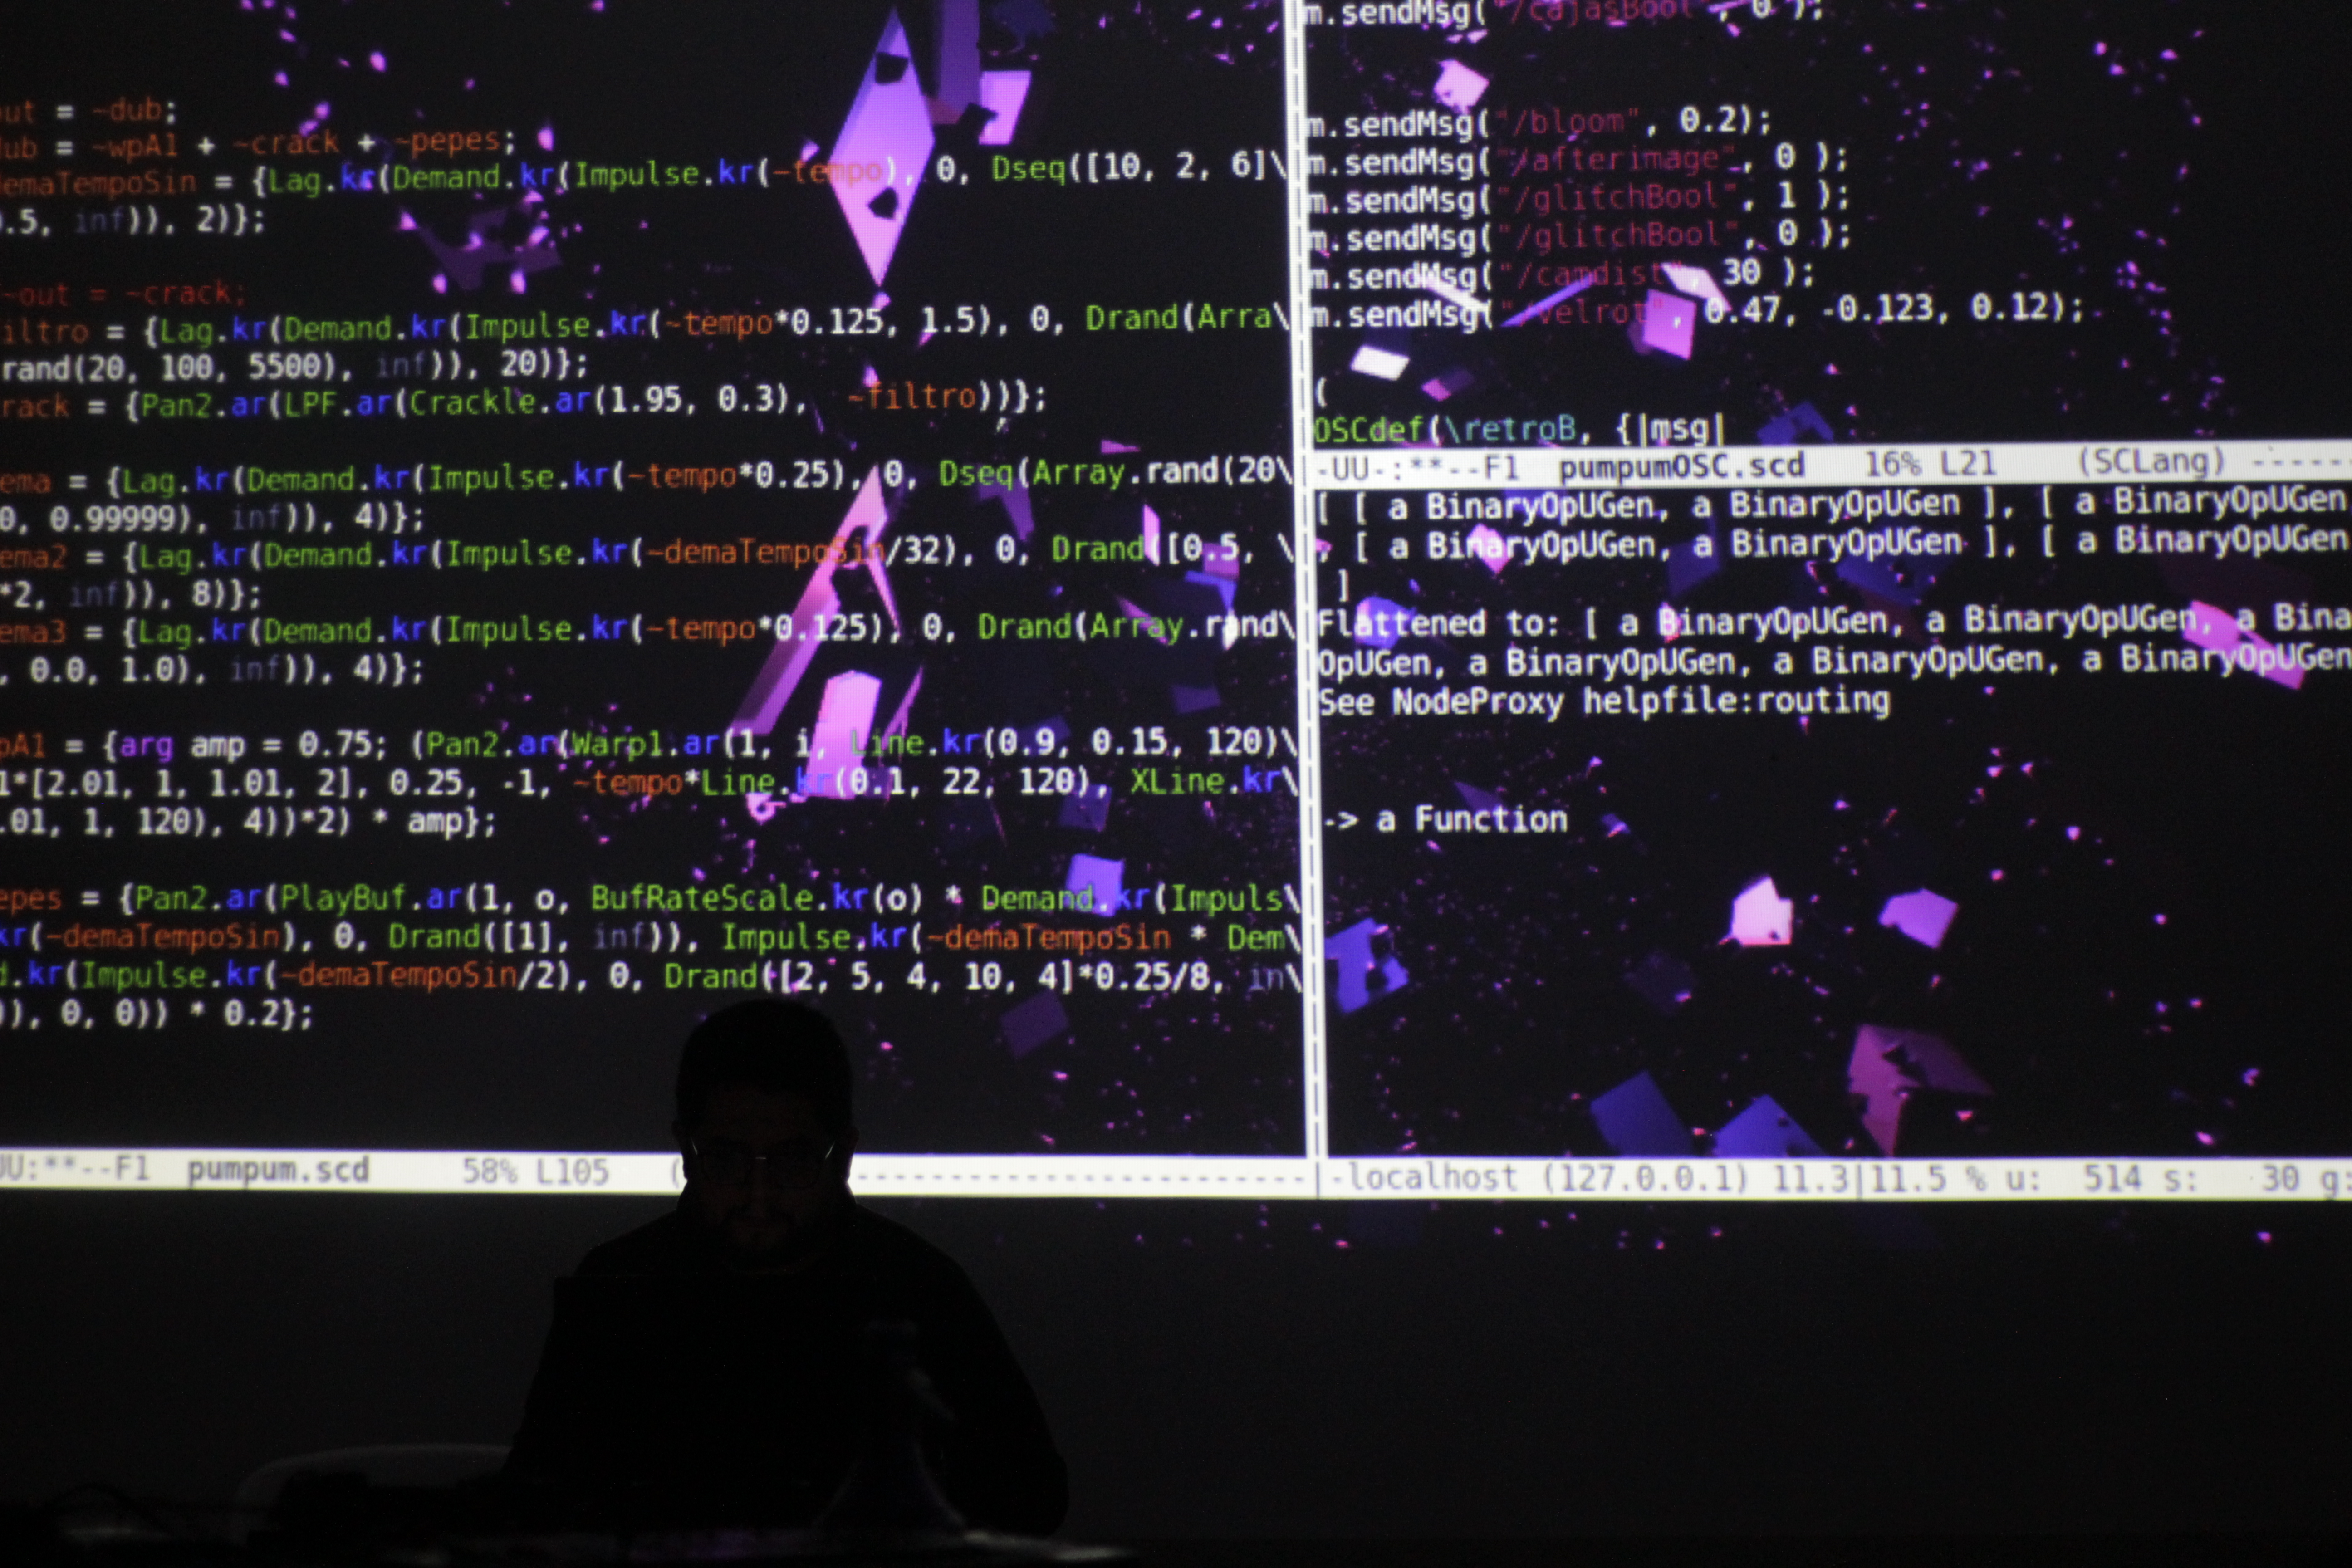
\includegraphics[width=\columnwidth]{../img/pumpum.JPG} 
%\caption[Concierto PUMPUM]{Presentación en el festival PUMPUM} % The text in the square bracket is the caption for the list of figures while the text in the curly brackets is the figure caption
%\label{fig:gallery} 
%\end{figure}

%\subsection{Concierto de clausura} % Este si podría ser relevante 

%Concierto virtual realizado en el marco del coloquio de alumnas del Programa de Posgrado en Música de la UNAM

%\begin{figure}[tb]
%\centering 
%\includegraphics[width=\columnwidth]{../img/col2.png} 
%\caption[Concierto coloquio]{Captura del concierto del Coloquio de alumnas \url{https://youtu.be/HwBTRQKr9Ps}.} % The text in the square bracket is the caption for the list of figures while the text in the curly brackets is the figure caption
%\label{fig:gallery} 
%\end{figure}

\section{PiranhaLab}

Otro antecedente de este proyecto es la práctica y reflexión planteada en colectivo por\textit{PiranhaLab}\footnote{``PiranhaLab es un laboratorio interdisciplinario que trabaja en las tripas del software''. \url{https://piranhalab.github.io/} (Consultado el \today)}.

%\subsection{Escritura de y con software}

%\subsection{Ciclo de Talleres}

El ciclo de talleres realizado en el Centro de Cultura Digital (CCD) en coparticipación con el Laboratorio de Tecnologías Libres\footnote{Actualmente Laboratorio de Tecnologías Compartidas} permitió plantear dos conclusiones que se heredan a \textit{Tres Estudios Abiertos}: La difuminación de la distinción usuario/desarrollador como una motivación para la escritura de software y la procuración de diversidad en la escritura de software en América Latina.

%\end{multicols}
%\vspace*{\fill}
\begin{figure} 
\includegraphics[width=\columnwidth]{../img/conversatorio.jpg} 
\caption[Conversatorio CCD]{Conversatorio organizado por PiranhaLab y el Laboratorio de Tecnologías Compartidas en el CCD. 2019.} % The text in the square bracket is the caption for the list of figures while the text in the curly brackets is the figure caption
\label{fig:gallery} 
\end{figure}
%\clearpage
%\begin{multicols}{1}
  %\raggedright
  
%\subsection{EDGES 2020}

La escritura de espacios para el ciclo de conciertos EDGES 2020 realizado por el Taller de Imágenes en Movimiento del Centro Multimedia (CMM) permitió la exploración de entornos tridimensionales inmersivos en el navegador en el contexto del encierro causado por la pandemia de COVID-19. Técnica y conceptualmente la escritura de estos espacios digitales influye en el presente proyecto. El artículo \textit{Panorama} \citep{panoramaArticulo} hace referencia de manera extensa al ecosistema de espacios y propuestas que también inciden en \textit{Tres Estudios Abiertos}.

% Esto se articula con las actividades colectivas de la sección casos 

Espacios inmersivos que estuvieron activos de manera simultánea. 

\section{Seminario Permanente de Tecnología Musical} 

El Seminario Permanente de Tecnología Musical (SPTM) es un espacio que se enmarca en el Posgrado en Música, específicamente en la línea de tecnología musical. Parte de las reflexiones de este proyecto de investigación se han abordado ahí y definitivamente se relacionan con investigaciones terminadas o en curso. La participación en este seminario permitió vislumbrar el mapa de investigaciones que se realizan en el Posgrado en Música de la UNAM y en específico, las posibles líneas de investigación que también forman parte del contexo en el que se inscribe esta investigación.

%\subsection{Transferencias Aurales}

Una de las primeras actividades que se realizaron en el marco de este seminario fue el Encuentro Latinoamericano de Música y Tecnología \textit{Transferencias Aurales} que tuvo lugar del 8 al 12 de noviembre de 2021.

%\subsection{Panorama} 

El ciclo de conciertos EDGES 2020 abrió posibilidades de reflexión a partir de la escritura de programas. Estas reflexiones fueron puestas a discusión en un espacio que consolidó una serie de artículos que conforman el libro \textit{Algoritmos Arruinados}. 

%\end{multicols}
%\vspace*{\fill}
\begin{figure} 
\includegraphics[width=\columnwidth]{../img/figura7.png} 
\caption[Distopía - Edges 2020]{Espacio diseñado para Distopía. ZGAMU (Música), LVSTVCVR(visuales e imágenes) y PiranhaLab (Diseño de espacio 3d)} % The text in the square bracket is the caption for the list of figures while the text in the curly brackets is the figure caption
\label{fig:gallery} 
\end{figure}
%\clearpage
%\begin{multicols}{1}
  %\raggedright
  
%\subsection{Semestre 2023-I}

% El trabajo con código ha sido preponderante. 

% \printendnotes


